\clearpage
\section{A descriptive fit to the rapid oscillations}
The late peak contains repeated sharp rises and falls. A single sinusoid does not describe their shape well. To visualize this structure, the interval $1536\leq t\leq1664$ is fitted with a slowly varying baseline and four harmonics:
\[
\widehat P(t)=c_0+c_1\tau+
\sum_{k=1}^{4}\left[(a_k+b_k\tau)\cos(2\pi kfu)
+(d_k+e_k\tau)\sin(2\pi kfu)\right],
\qquad u=t-1600,\quad\tau=u/64.
\]
A harmonic is an oscillation at an integer multiple of a base frequency. Combining harmonics allows sharper peaks than one sine wave; the linear amplitude factors allow their height to change across this local interval. The 18 linear coefficients are fitted by least squares, while the base frequency is optimized in $0.084\leq f\leq0.091$, guided by the sampled spectrum. This frequency interval is a modelling choice, not a physical constraint.
\begin{center}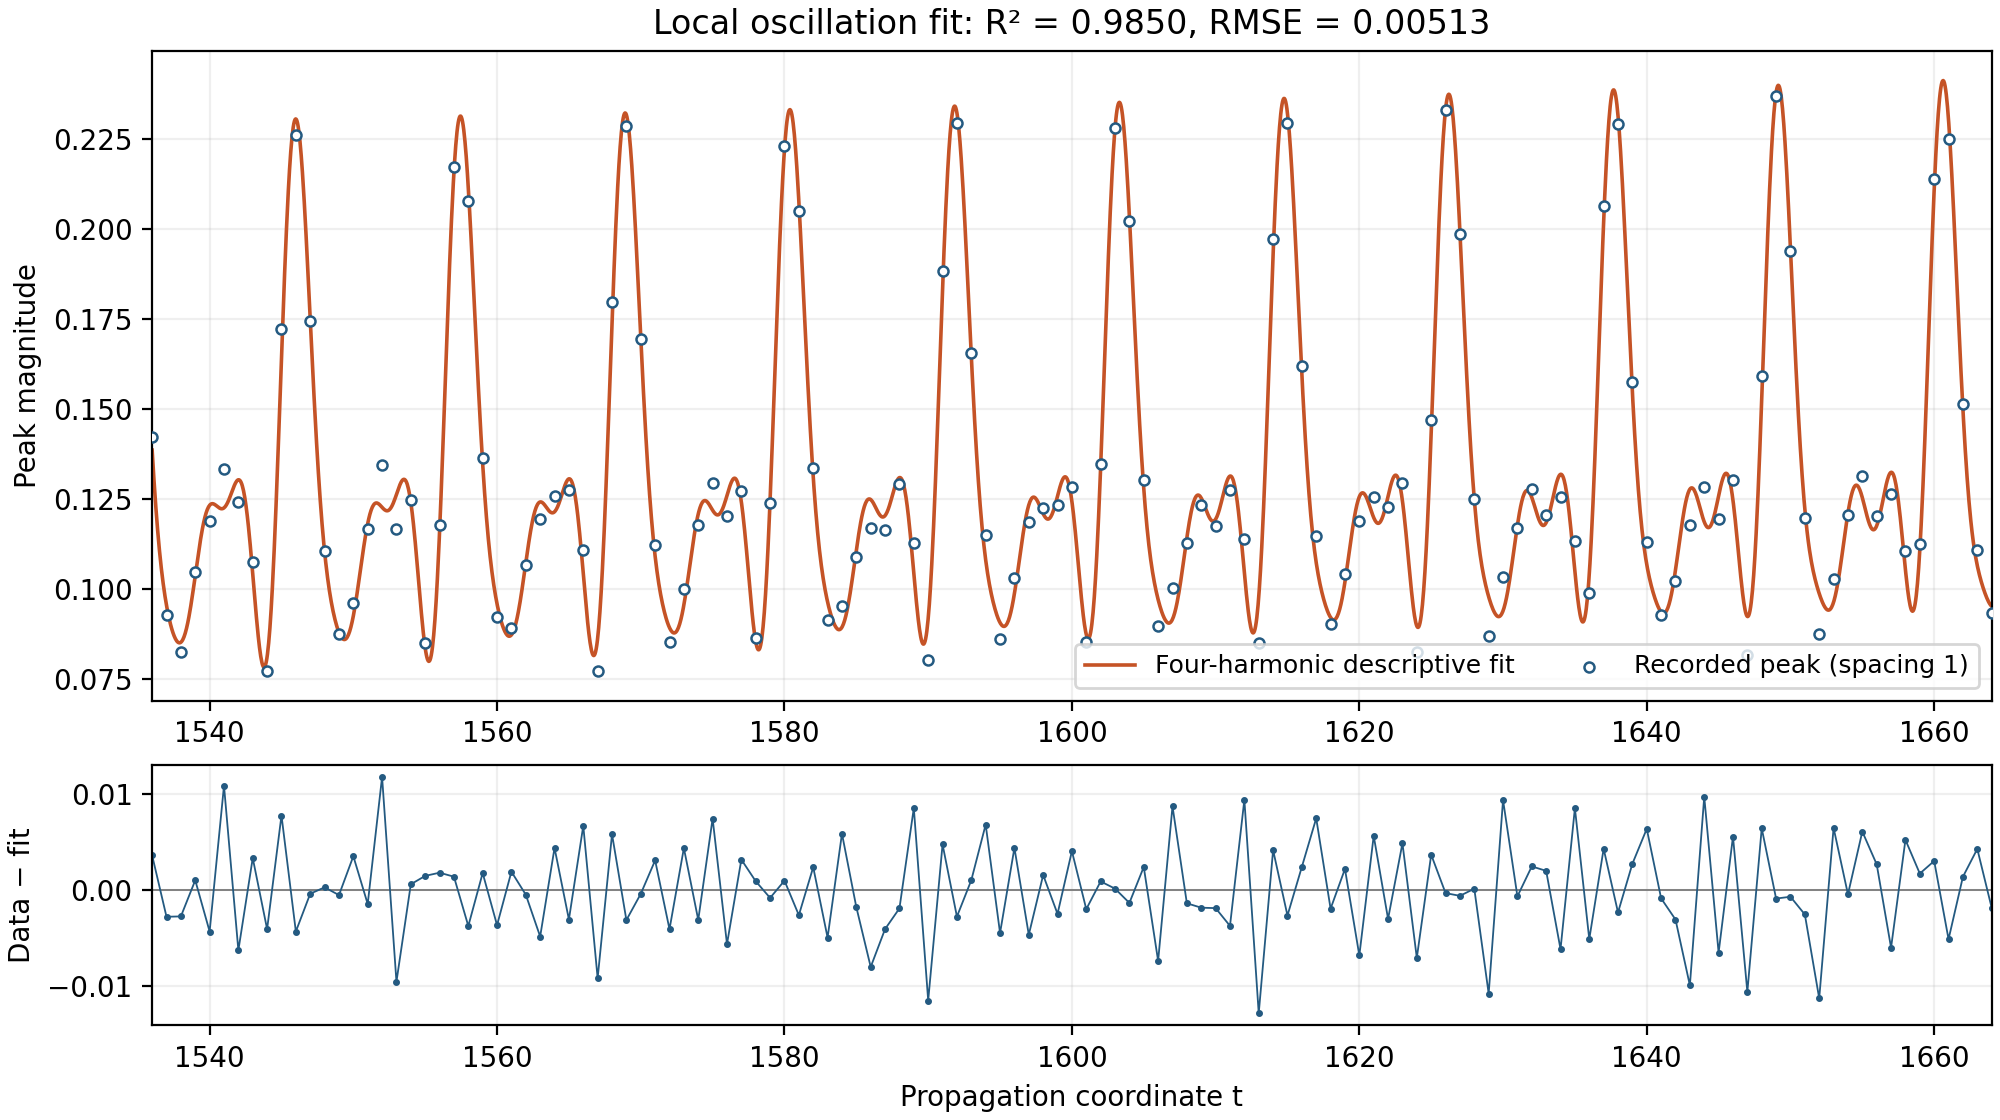
\includegraphics[width=\linewidth]{oscillation_fit.png}\end{center}
\noindent\textbf{Figure 3.} Recorded peak values and the local oscillatory fit, with residuals beneath. The smooth line approximates the sampled data; it is not a new PDE solution or a prediction outside this interval.

The fitted base period is $11.4821$, and its second harmonic has period $5.7411$. The refit on all 129 points has RMSE $0.00513$ and $R^2=0.9850$. These quantify local descriptive agreement, not long-time numerical accuracy.

Harmonic counts one through four were compared by withholding every fifth point. Their validation RMSEs were $0.03474$, $0.01802$, $0.00870$, and $0.00523$, respectively. Four harmonics were selected and then refitted using all points. Because these withheld points selected the model, they are not an independent final test. The fit uses 19 adjustable quantities including frequency. Sampling at unit intervals cannot rule out aliased higher frequencies or establish the exact continuous peak between records. Neither the fitted periods nor the high local $R^2$ establish a soliton, a decay exponent, or a globally periodic orbit.
